\documentclass{resonance}
\usepackage[T1]{fontenc}
\usepackage{braket}
\usepackage{dsfont}
\usepackage{xparse}
\usepackage{subfig}
\usepackage{hyperref}
\usepackage{tikz}
\usepackage{afterpage}
\usepackage{lmodern}
\hypersetup{
    colorlinks=true,
    linkcolor=blue,
    filecolor=magenta,      
    urlcolor=cyan,
    pdftitle={Overleaf Example},
    pdfpagemode=FullScreen,
    }

\begin{document}

\title{The Dance of Atoms}
\secondTitle{A primer on some fundamental concepts in Condensed Matter Physics}
\author{Debasish Panda}

\maketitle
%%\authorIntro is used to place the author's photo and an introduction about the author
%%photo goes into the includegraphics with width=2cm 
%%and a "\\" dividing the text and photo
%%the intro text box is drawn automatically
%%place \authorIntro  just before abstract
\authorIntro{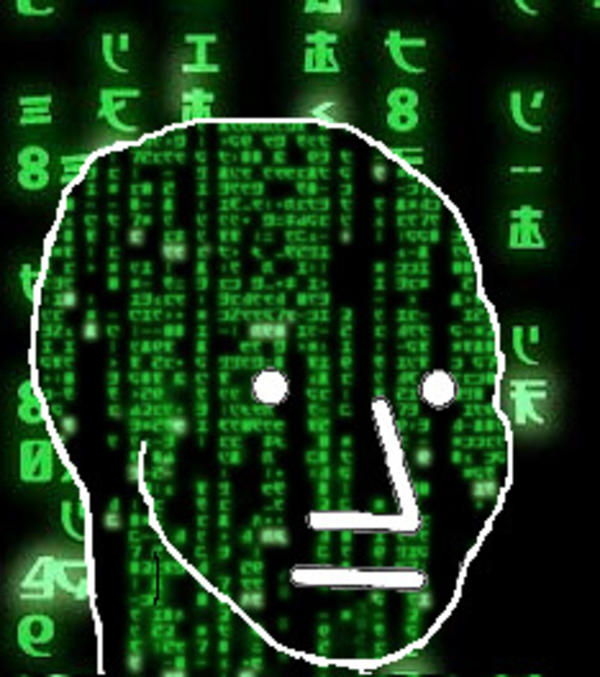
\includegraphics[width=2cm]{wojak_matrix.png}\\
Si vis pacem, para bellum}
%%abstract
\begin{abstract}
Semiconductor-based devices have become the lifeblood of modern civilisation, powering the tiniest microprocessor to the largest of the ICBMs. In our quest for smaller and still smaller transistors, we have now hit a fundamental barrier beyond which deterministic Newtonian mechanics is helpless and quantum mechanics reigns with all its glory of probabilistic chaos. This calls immediately for a fundamental understanding of the quantum mechanical nature of such beyond-Moore devices, viz., \textit{quantum devices}. This article is devoted to a brief exploration of such concepts, starting from simple toy models of quantum condensed matter systems---reviewing the tight-binding ansatz, physics of quantum bands, second quantization---and touching upon the state-of-the-art in modern condensed matter---quantum topology and topological electronics.  
\end{abstract}

\monthyear{February 2024}
\artNature{GENERAL ARTICLE}

\section{Second Quantization}

Before we begin our incursion into the so-called 'second quantization', we need to appreciate the reason why the need for second quantization arose. The properties of quantum condensed matter systems and, by extension, that of real materials are controlled by the \textit{collective behaviour} of electrons in the presence of some background potential due to an underlying crystal lattice. This statement, in fact, is a simpler rendition of the Bohr-Oppenheimer approximation. So, what factors do we need to consider during the analysis of a condensed matter system?
\begin{itemize}
    \item Focus on electrons and their collective dynamics
    \item Electrons are free to move from one orbital to another (tunnelling/hopping)
    \item They are subject to a background potential from the lattice
    \item They can interact with each other due to Coulomb repulsion
\end{itemize}
The question remains, how do we formulate the Hamiltonian for many-body systems? How do we encode anti-symmetry of fermions into this many-particle wavefunction? And most importantly, how do we find out the eigenstates/eigenvalues of momentum and/or energy of the system?  \par

So, how do we encode fermionic anti-symmetry in many-particle wavefunctions? \\
Consider a single-particle quantum state $\phi_{\nu}(\vec{r})$, where $\nu$ refers to labels for the quantum state. The basis for a two-particle system is then given by 

\begin{equation*}
    \psi(\vec{r_{1}}, \vec{r_{2}}) = \frac{1}{\sqrt{2}}[\phi_{\nu_{1}}(\vec{r_{1}}) \phi_{\nu_{2}}(\vec{r_{2}}) - \phi_{\nu_{1}}(\vec{r_{2}}) \phi_{\nu_{2}}(\vec{r_{1}})]
\end{equation*}

This basis satisfies the anti-symmetry property, and also, there happens to be a less verbose manner through which we can express such wavefunctions - Slater's determinants. \\
For a generalized N-particle system such that the basis states are perfectly anti-symmetric under exchanging the labels of any two particles, the wavefunction can be expressed as

\begin{equation*}
    \psi(\vec{r_{1}}, \vec{r_{2}},..., \vec{r_{N}}) = \frac{1}{\sqrt{N!}} \begin{bmatrix}
        \phi_{\nu_{1}}(\vec{r_{1}}) & \phi_{\nu_{2}}(\vec{r_{1}}) & ... & \phi_{\nu_{N}}(\vec{r_{1}}) \\
        \phi_{\nu_{1}}(\vec{r_{2}}) & \phi_{\nu_{2}}(\vec{r_{2}}) & ... & \phi_{\nu_{N}}(\vec{r_{2}}) \\
        . & . &  & . \\
        . & . &  & . \\
        . & . &  & . \\
        \phi_{\nu_{1}}(\vec{r_{N}}) & \phi_{\nu_{2}}(\vec{r_{N}}) & ... & \phi_{\nu_{N}}(\vec{r_{N}})
    \end{bmatrix}
\end{equation*}

The 'first quantization' principle cannot be used to satisfactorily explain condensed matter systems since calculations become cumbersome and expensive as the number of particles in the system increases, and the representation requires the number of particles, $N$, to be fixed. As $N$ approaches the limit associated with statistical physics, $N$ is allowed to fluctuate as per the grand canonical ensemble. Second quantization or occupation number formalism is the standard way in which many-particle QM is formulated. It is based on the algebra of ladder operators. 
\begin{itemize}
    \item Second quantization provides a compact way of representing the many-body space of excitations.
    \item Properties of operators encoded in a single set of commutation/anti-commutation relations rather than in some explicit Hilbert space representation.
    \item Formalism greatly simplifies actual calculations for purposes of simulation.
\end{itemize}

\subsection{Single qubit system}
Qubit states are labelled by their occupation numbers, $\ket{n}$, with $n$ = 0, 1 being a quantum number corresponding to fermionic occupation. The local Hilbert space, $\mathcal{H}$, is 2-dimensional, being spanned by \{$\ket{0}$, $\ket{1}$\}. The properties of the elements of $\mathcal{H}$ have been tabulated as follows.
\begin{itemize}
    \item \textbf{Orthonormality}\\
    $\braket{0|0} = \braket{1|1} = 1$; $\braket{1|0} = \braket{0|1} = 0$
    
    \item \textbf{Ladder operators}\\
    Creation operator, $\hat{c}^{\dagger} \ket{0} = \ket{1}$; Annihilation operator, $\hat{c}\ket{1} = \ket{0}$\\
    However, $\hat{c} \ket{0} = \ket{0}$, $\hat{c}^{\dagger} \ket{1} = \ket{0}$\\
    $\hat{c}^{\dagger} = \ket{1}\bra{0}$, $\hat{c} = \ket{0}\bra{1}$

    \item \textbf{Hermitian conjugation}\\
    $(\hat{c}^{\dagger})^{\dagger} = (\ket{1}\bra{0})^{\dagger} = \ket{0}\bra{1} = \hat{c}$; $(\hat{c})^{\dagger} = (\ket{0}\bra{1})^{\dagger} = \ket{1}\bra{0} = \hat{c}^{\dagger}$\\
    $\hat{c}$ and $\hat{c}^{\dagger}$ are not Hermitian operators but rather Hermitian conjugates of each other.

    \item \textbf{Identity operator}\\
    $\mathds{1} = \ket{0}\bra{0} + \ket{1}\bra{1}$ is defined s.t. $\mathds{1}\ket{\psi} = \ket{\psi}$

    \item \textbf{Number operators}\\
    Define a number operator, $\hat{n} = \hat{c}^{\dagger} \hat{c}$ ($\hat{n}$ is Hermitian) \\
    $\hat{n}\ket{0} = \hat{c}^{\dagger} \hat{c} \ket{0} = 0 \cdot \ket{0} = 0$\\
    $\hat{n}\ket{1} = \hat{c}^{\dagger} \hat{c} \ket{1} =  \hat{c}^{\dagger} \ket{0} = \ket{1}$\\
    Hence, $\hat{n}\ket{n} = n\ket{n}$, where $n$ is the number of $e^{-}$s in the system. \\
    The states $\ket{0}$ and $\ket{1}$ are eigenstates of the number operator, $\hat{n}$. The eigenvalue $n$ is the so-called occupation number (it classifies as a quantum number).

    \item \textbf{Hamiltonian}\\
    $\hat{H} = \mathcal{E} \hat{n}$; where $\mathcal{E}$ represents the single particle energy of state. Additional terms aren't needed since it turns out that $\hat{n}$ is idempotent, i.e., $\hat{n}^{2} = \hat{n}$. \\
    The Hamiltonian and the number operators commute, so the occupation number basis \{$\ket{0}$, $\ket{1}$\} are indeed eigenstates of $\hat{H}$.
    
    \item \textbf{Anti-commutation relations}\\
    This is the real deal for us since it encodes the operator algebra.\\
    $\hat{c}^{\dagger} \hat{c} \mathds{1} = \ket{1}\bra{1}$; $\hat{c} \hat{c}^{\dagger} \mathds{1} = \ket{0}\bra{0}$\\
    $\implies (\hat{c}^{\dagger} \hat{c} + \hat{c} \hat{c}^{\dagger}) \mathds{1} = \ket{0}\bra{0} + \ket{1}\bra{1} = \mathds{1}$ $\implies \{\hat{c}^{\dagger}, \hat{c}\} = \mathds{1}$ \\
    Similar anti-commutation relations can be written for $\hat{c}$ and $\hat{c}^{\dagger}$: $\{\hat{c}, \hat{c}\} = \{\hat{c}^{\dagger}, \hat{c}^{\dagger}\} = 0$  
\end{itemize}

\subsection{Two qubit system}
Consider two distinct orbitals, $\{\ket{0}_{1}, \ket{1}_{1}\}$ and $\{\ket{0}_{2}, \ket{1}_{2}\}$. We have already established the algebraic properties for the single qubit system, but what about operations such as $\{\hat{c}_{i}^{\dagger}, \hat{c}_{j}^{\dagger}\}$; $i \neq j$?\\
The 4-dimensional state space of a 2-qubit system is spanned by $\{\ket{0}_{1} \otimes \ket{0}_{2}, \ket{0}_{1} \otimes \ket{1}_{2}, \ket{1}_{1} \otimes \ket{0}_{2}, \ket{1}_{1} \otimes \ket{1}_{2}\}$. \\
The Hilbert space for a $N$-particle system is defined by the product of $N$ single-particle Hilbert spaces. 

\begin{equation*}
    \mathcal{H}^{N} = \mathcal{H \otimes H \otimes H ...} = \bigotimes_{i = 1}^{N} \mathcal{H}_{i}
\end{equation*}

Thus, the $N$-particle states would be defined as a linear superposition of the basis states of the Hilbert space, $\mathcal{H}^{N}$. The \textit{Fock space} ($\mathcal{F}$) constitutes the vector space for any number of particles and is, thus, defined as 

\begin{equation*}
    \mathcal{F} = \bigoplus _{N = 0}^{\infty} \mathcal{H}^{N}
\end{equation*}

Now, consider each of the wavefunctions spanning the state space of the 2-qubit system.

\begin{equation}
\begin{aligned}
    \ket{\psi}_{1} &= \ket{0}_{1} \otimes \ket{0}_{2} = \ket{vac}\\
    \ket{\psi}_{2} &= \ket{0}_{1} \otimes \ket{1}_{2} = \hat{c}_{2}^{\dagger}\ket{vac}\\
    \ket{\psi}_{3} &= \ket{1}_{1} \otimes \ket{0}_{2} = \hat{c}_{1}^{\dagger}\ket{vac}\\
    \ket{\psi}_{4} &= \ket{1}_{1} \otimes \ket{1}_{2} = \hat{c}_{1}^{\dagger} \hat{c}_{2}^{\dagger}\ket{vac}
\end{aligned}
\end{equation}

Now, consider the permutation operator, $\hat{P}_{12}$, which swaps the labels of particles 1 and 2. Using the property of wavefunction asymmetry of fermions under interchange of particles, we can thus claim that

\begin{equation}
\begin{aligned}
    \hat{P}_{12} \ket{\psi_{4}} &= -\ket{\psi_{4}} \\
    \hat{P}_{12} (\hat{c}_{1}^{\dagger} \hat{c}_{2}^{\dagger}\ket{vac}) &= \hat{c}_{2}^{\dagger} \hat{c}_{1}^{\dagger}\ket{vac} = -\hat{c}_{1}^{\dagger} \hat{c}_{2}^{\dagger}\ket{vac}\\
    (\hat{c}_{1}^{\dagger} \hat{c}_{2}^{\dagger} + \hat{c}_{2}^{\dagger} \hat{c}_{1}^{\dagger})\ket{vac} &= 0 \implies \{\hat{c}_{1}^{\dagger}, \hat{c}_{2}^{\dagger}\} = 0
\end{aligned}
\end{equation}

Similarly, $\{\hat{c}_{1}, \hat{c}_{2}\} = \{\hat{c}_{1}, \hat{c}_{2}^{\dagger}\} = 0$. Compiling these results formally,

\begin{equation}
    \{\hat{c}_{i}, \hat{c}_{j}^{\dagger}\} = \delta_{ij}
\end{equation} 

We are now in a position to define the generalized state of a $N$-particle system. 

\begin{equation*}
    \ket{n_{1}, n_{2},..., n_{N}} = \ket{n_{1}} \otimes \ket{n_{2}} \otimes... \otimes \ket{n_{N}} = \bigotimes _{i = 1}^{N} \ket{n_{i}} = \prod_{i = 1}^{N}(\hat{c}_{i}^{\dagger})^{n_{i}} \ket{vac} 
\end{equation*}

Note that we made quite a strong statement: for \textit{any N},  the \textit{N}-body wavefunction can be generated by an application of a set of \textit{N}-independent operators to a unique vacuum state. Using some simple mathematical manipulations, it can be shown that for $i \neq j$, $[\hat{n}_{i}, \hat{c}_{j}^{\dagger}] = 0$, i.e., they commute. One could take this even further and show that the occupation number basis states are indeed the eigenstates of the number operator, $\hat{n}_{j}$, with eigenvalue $n_{j}$. 

\begin{equation}
    \hat{n}_{j} \ket{n_{1}, n_{2}, n_{3},..., n_{N}} = n_{j}\ket{n_{1}, n_{2}, n_{3},..., n_{N}}
\end{equation}

The total number of electrons in the N-particle system is then given by the number operator, $\hat{N} = \sum_{i} \hat{n}_{i}$, s.t. $N = \sum_{i}n_{i}$. \\

\leftHighlight{Canonical fermionic anti-commutation relations are at the heart of operator algebra}

\subsection{Change of basis}
Suppose we wish to transform the creation/annihilation operators $\hat{c}_{\lambda}^{\dagger}$ corresponding to the basis set $\{\ket{\lambda}\}$ to a different basis set, $\{\ket{\Tilde{\lambda}}\}$. What will be the functional form of the new creation/annihilation operators, $\hat{c}_{\Tilde{\lambda}}^{\dagger}$? \par
Using the property of resolution of the identity operator, $\mathds{1} = \sum_{\lambda = 0}^{\infty} \ket{\lambda}\bra{\lambda}$, one can establish the relations, $\ket{\Tilde{\lambda}} = \sum_{\lambda}\ket{\lambda}\braket{\lambda|\Tilde{\lambda}}$. The transformation laws are then given by,

\begin{equation}
    \hat{c}_{\Tilde{\lambda}}^{\dagger} = \sum_{\lambda}\braket{\lambda|\Tilde{\lambda}} \hat{c}_{\lambda}^{\dagger}
\end{equation}

\begin{equation}
    \hat{c}_{\Tilde{\lambda}} = \sum_{\lambda}\braket{\Tilde{\lambda}|\lambda} \hat{c}_{\lambda} 
\end{equation}

\subsection{Representation of operators}
Single particle or one-body operators $\hat{\mathcal{O}_{1}}$ acting in a \textit{N}-particle Hilbert space, $\mathcal{H}^{N}$, generally take the form $\hat{\mathcal{O}_{1}} = \sum_{n = 1}^{N}\hat{o}_{n}$, where $\hat{o}_{n}$ is an ordinary single-particle operator acting on the \textit{n}-th particle. A typical example is the kinetic energy operator $\hat{T} = \sum_{n}\frac{\hat{p}_{n}^{2}}{2m}$, where $\hat{p}_{n}$ is the momentum operator acting on the \textit{n}-th particle. Since we have seen that, by applying field operators to the vacuum space, we can generate the Fock space in general and any \textit{N}-particle Hilbert space in particular, it must be possible to represent any operator $\hat{\mathcal{O}_{1}}$ using the set of creation/annihilation operators. Here, we present the formal representation of a one-body operator using second quantization principles,

\begin{equation}
    \hat{\mathcal{O}_{1}} = \sum_{\lambda \mu \nu}\braket{\mu | \lambda}o_{\lambda}\braket{\lambda | \nu}\hat{c}^{\dagger}_{\mu} \hat{c}_{\nu} = \sum_{\mu \nu}\braket{\mu|\hat{o}|\nu}\hat{c}^{\dagger}_{\mu} \hat{c}_{\nu}
\end{equation}

Formally, the one-body operator, $\hat{\mathcal{O}_{1}}$, scatters a particle from a state $\nu$ into a state $\mu$ with probability amplitude $\braket{\mu|\hat{o}|\nu}$. \par
Two-body operators $\hat{\mathcal{O}_{2}}$ are needed to describe \textit{pairwise interactions} between particles. Although pair-interaction potentials are
straightforwardly included in classical many-body theories, their embedding into conventional many-body quantum mechanics is made awkward by particle indistinguishability. Here again, we present the formal representation of a two-body operator using second quantization principles without providing a derivation for the same.

\begin{equation}
    \hat{\mathcal{O}_{2}} = \sum_{\lambda \lambda^{\prime} \mu \mu^{\prime}} \braket{\mu, \mu^{\prime}|\mathcal{O}_{2}|\lambda, \lambda^{\prime}} \hat{c}_{\mu^{\prime}}^{\dagger} \hat{c}_{\mu}^{\dagger} \hat{c}_{\lambda} \hat{c}_{\lambda^{\prime}}
\end{equation}

\section{Bloch's Theorem}
Periodic potentials are important in condensed matter physics, and we will be using the Bloch wavefunctions generously during the analysis of toy models. Secondly, periodic potentials will give us our first examples of Hamiltonian systems with symmetry, and they will serve to illustrate certain general principles of such systems. \par
We wish to solve the one-dimensional Schrödinger equation,

\begin{equation}
    -\frac{\hbar^{2}}{2m}\psi^{\prime \prime} + V(x) \psi = E \psi
\end{equation}

where the potential is assumed to be spatially periodic,

\begin{equation}
    V(x+a) = V(x)
\end{equation}

Here \textit{a} is the lattice spacing or spatial period of the 1-D lattice. No further assumptions need be made about the behaviour of \textit{V(x)} within any period apart from its periodicity. \par
Next, we shall make a strong assumption that there is a super-symmetry that rides over the good ole periodicity of the lattice points such that the lattice repeats itself after \textit{N} lattice spacings. This is equivalent to imposing a periodic/circular boundary condition on the solutions to the Hamiltonian. \par
We introduce the translation operator, $T(a)$, which has the effect of displacing the wave function by the lattice spacing \textit{a} along the x-axis. 

\begin{equation}
    T(a) \psi(x) = \psi (x-a)
\end{equation}

Functionally, the translation operator is given by,

\begin{equation}
    T(a) = e^{-\frac{iap}{\hbar}}
\end{equation}

An easy check will ascertain that this operator commutes with both kinetic energy, as well as potential energy operators. This means that \textit{T(a)} commutes with the entire Hamiltonian, 

\begin{equation}
    [T(a), H] = 0
\end{equation}

Put more generally, \textit{H} commutes with any power of \textit{T(a)}, \textit{$T(a)^{n} = T(na)$}, which is to say that it commutes with the entire group of symmetry operations generated by \textit{T(a)}. \par
The fact that \textit{H} and \textit{T(a)} commute provides us a powerful tool to determine the eigenfunctions of \textit{H}. More often than not, it is hard to find the eigenfunctions of \textit{H}, but much easier to find those for the translation operator. Since we now know the eigenfunctions of the translation operator, it makes the search for the eigenfunctions of \textit{H} easier since they are a subset of the eigenspace of \textit{T(a)}. \par
\rightHighlight{An interesting offshoot of the Bloch wavefunction is the concept of 'crystal momentum', which does not represent the momentum of the electron in real space but rather encapsulates the effect of the net external potential acting on it without having to worry about the internal forces.}
Since \textit{T(a)} is unitary, its eigenvalue $\tau$ must be a phase factor, $\tau = e^{-i\theta}$. The angle $\theta$ characterizes the eigenvalues of \textit{T(a)} and may be restricted to the range $-\pi < \theta \leq \pi$. It is conventional to write this angle in the form $\theta = ka$, where \textit{k} is a quantity with dimensions of wave number,
which characterizes the eigenvalue. We now have,

\begin{equation}
    T(a) \psi_{k}(x) = \psi_{k}(x-a) = e^{-ika}\psi_{k}(x)
\end{equation}

Equivalently, we can write this as,

\begin{equation}
\label{eq:bloch wavefunction}
    \psi_{k}(x+a) = e^{ika}\psi_{k}(x)
\end{equation}

Now we are faced with a dilemma - for any given value of \textit{k}, there are functions $\psi_{k}$ which satisfy \ref{eq:bloch wavefunction}, so the spectrum of \textit{T(a)} is the entire unit circle in the complex plane. Furthermore, the number of such functions for any value of $e^{-ika}$ is infinite, so the eigenvalues are infinite-fold degenerate and the eigenspaces of \textit{T(a)} are infinite-dimensional. This would render the entire analysis using translation operators inconsequential since it was asserted that this approach would help limit the space in which we have to search for the eigenfunctions of \textit{H}. This is exactly where the initial boundary condition assuming a super-symmetry comes into play. In case the lattice repeats itself after \textit{N} lattice spacings, the single-valuedness of the wavefunction requires

\begin{equation}
    \psi(x+Na) = \psi(x)
\end{equation}

so the eigenvalues of \textit{T(a)} are phase factors of the form $e^{-\frac{2n\pi i}{N}}$, for \textit{n = 0,..., N-1}. In this case, the spectrum of \textit{T(a)} is discrete, although each eigenvalue is still infinite-fold degenerate. Rather than $\psi_{k}(x)$, it is often easier to work with a function $u_{k}(x)$, defined by

\begin{equation}
    \psi_{k}(x) = \psi_{k}(x) u_{k}(x)
\end{equation}

where $u_{k}$ is periodic, $u_{k}(x+a) = u_{k}(x)$. \textit{Bloch's theorem} states that since \textit{H} commutes with \textit{T(a)}, \textit{H} possesses eigenfunctions which are of the form of $\psi_{k}(x)$, that is, $e^{ikx}$ times a periodic function $u_{k}(x)$. 


\section{Tight Binding Models}

Before moving in to consider Hamiltonians for a system of interacting particles, we wish to propose model Hamiltonians for non-interacting fermionic systems. Consider, for example, the free electron gas, with electrons occupying quantum states $\ket{k} = \ket{n_{k}}$. The Hamiltonian is given by,

\begin{equation}
    \hat{H} = \sum_{k}\mathcal{E}_{k} \hat{c}^{\dagger}_{k} \hat{c}_{k} = \sum_{k}\mathcal{E}_{k} \hat{n}_{k}
\end{equation}

where $\mathcal{E}_{k}$ represents the single-particle state of energy corresponding to the P.E. associated with orbital $\ket{k}$. It is straightforward to show that number operator $\hat{n}_{k}$ commutes with $\hat{H}$; that is, the set $\{n_{k}\}$ is conserved by $\hat{H}$ and can be classified as the so-called \textit{good} quantum numbers. \par

\begin{equation}
    \hat{H}\ket{n_{1}, n_{2},..., n_{N}} = E_{n_{1}, n_{2},..., n_{N}}\ket{n_{1}, n_{2},..., n_{N}}
\end{equation}

where $E_{n_{1}, n_{2},..., n_{N}} = \sum_{i}\mathcal{E}_{i} n_{i}$. \par
Now, we shall introduce an additional layer of complexity to the problem by accounting for the interaction between fermionic particles constituting the system. The modified Hamiltonian is then expressed as,

\begin{equation}
    \hat{H} = \sum_{i}\mathcal{E}_{i} \hat{c}_{i}^{\dagger} \hat{c}_{i} + \sum_{i \neq j}t_{ij} \hat{c}_{i}^{\dagger} \hat{c}_{j}
\end{equation}

where $t_{ij}$ is the tunnelling matrix element corresponding to the tunnelling/hopping of an electron from orbital $\ket{i}$ to orbital $\ket{j}$, s.t. $\braket{i|\hat{H}|j} = t_{ij}$. Additionally, since the Hamiltonian is Hermitian, it places a restriction on the elements of the tunnelling matrix, namely, $t_{ij} = t_{ji}^{*}$. Such tight-binding models can be used to describe many condensed matter and molecular systems, which include scenarios such as a lattice where atomic orbitals overlap, and $e^{-}$s can tunnel/hop from one orbital to another. \par

\begin{figure}[!t]
\caption{\textit{The $p_{z}$ orbitals of the respective carbon atoms in benzene interact with their nearest neighbours, forming a delocalized network of pi-$e^{-}$s}}\label{benzene}
\centering
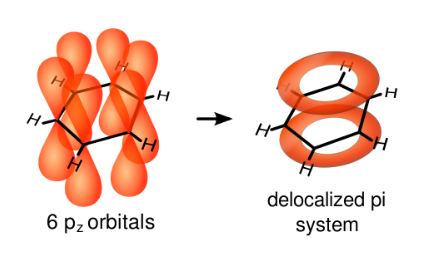
\includegraphics[scale=0.7]{benzene.png}
\end{figure}

Benzene provides an excellent toy model for studying the application of tight-binding models. The $p_{z}$ orbitals interact with only their nearest neighbours, greatly simplifying the expression for the Hamiltonian associated with the $\pi$-bonded network.

\begin{equation}
    \hat{H}_{\pi} = \mathcal{E}\sum_{i = 1}^{6}\hat{c}_{i}^{\dagger} \hat{c}_{i} + t\sum_{i = 1}^{6} (\hat{c}_{i}^{\dagger} \hat{c}_{i+1} + \hat{c}_{i+1}^{\dagger} \hat{c}_{i})
\end{equation}

The situation is somewhat similar in the case of graphene, which consists of stacked 2-D hexagonal lattices of carbon atoms. The Hamiltonian for the $\pi$-bonded network is given by,

\begin{equation}
    \hat{H}_{\pi} = \mathcal{E}\sum_{i}\hat{c}_{i}^{\dagger} \hat{c}_{i} + t\sum_{i,j} (\hat{c}_{i}^{\dagger} \hat{c}_{j} + \hat{c}_{j}^{\dagger} \hat{c}_{i})
\end{equation}

where $i, j$ constitute the indices of nearest neighbours on the hexagonal lattice. 


\section{Electronic Bandstructure}

Using the results of the tight-binding model (or, more appropriately, the approximations used in the tight-binding model) and that of Bloch's theorem, we can analyse the electronic band structure for a 1-D chain of atoms, followed by increasingly complex variations of the same. \par
Consider a linear chain of identical hydrogenic atoms ($ns$ orbitals) with individual lattice points separated by a distance $a$. From the LCAO theory, the generalized wavefunction of the system can be expressed as:

\begin{equation}
    \psi = c_{1}\phi_{1} + c_{2}\phi_{2} + c_{3}\phi_{3} + ... = \sum_{n}c_{n}\phi_{n} = \sum_{n}e^{ikx_{n}}\phi_{n}
\end{equation}

where $x_{n}$ is the position of the $n$th atom. The atoms, being identical, contribute equally to the LCAO in terms of their wavefunction amplitude but with different phase factors to account for their periodic distribution. More formally, this idea is captured via Bloch's theorem, which presents a generalised wavefunction for particles in a periodic lattice:

\begin{equation}
    \psi_{k}(\vec{r}) = e^{i\vec{k}\cdot \vec{r}}u_{k}(\vec{r})
\end{equation}

where $u_{k}(\vec{r})$ is called the \textit{cell function}, and represents atoms in the unit cell. In our case, the Bloch wavefunction is given by,

\begin{equation}
    \psi_{k} = \sum_{n=1}^{N} e^{ikna}\phi_{n}
\end{equation}

The Bloch wavefunction incorporates the real-space symmetry of the lattice into the $k$-space in the sense that for $k > \frac{\pi}{a}$, the wavefunction merely acquires a global phase, and this does not affect the expectation value of measurables. The energy eigenvalue of the Bloch wavefunction serves as a direct measure of the $E-k$ relationship and is given by,

\begin{equation}
    E = \frac{\int \psi_{k}^{\dagger} \mathcal{H}\psi_{k} dx}{\int \psi_{k}^{\dagger} \psi_{k} dx}
\end{equation}

Note that we have abandoned the \textit{bra-ket} notation since I found the conventional method to be more intuitive in this case. I might later consider adding a similar analysis but using the \textit{bra-ket} notation. Now, 

\begin{equation}
    \int \psi_{k}^{\dagger}\mathcal{H}\psi_{k}dx = \sum_{n=1}^{N} \sum_{m=1}^{N}e^{i(n-m)ka} \int \phi_{m}^{\dagger}\mathcal{H}\phi_{n} dx
\end{equation}

Applying the constraints of the tight-binding approximation, the integral term involved in RHS can be simplified into three distinct cases: $\alpha$ if $m = n$, i.e., the potential energy corresponding to each lattice site, $\beta$ if $|m-n| =1$, i.e., the lattice sites correspond to nearest neighbours, and $0$ otherwise. 

\begin{equation}
    \int \psi_{k}^{\dagger}\mathcal{H}\psi_{k}dx = N(\alpha + \beta[e^{-ika}+e^{ika}]) = N(\alpha + 2\beta \text{cos}(ka))
\end{equation}

\begin{equation}
    \int \psi_{k}^{\dagger}\psi_{k}dx = \sum_{n=1}^{N} \sum_{m=1}^{N}e^{i(n-m)ka} \int \phi_{m}^{\dagger}\phi_{n} dx = N
\end{equation}

since the integral term in the RHS evaluates as null unless $m = n$. Hence, the energy eigenvalue is given by:

\begin{equation}
    E_{k} = (\alpha + 2\beta \text{cos}(ka))
\end{equation}

As pointed out earlier, for values of $k > \frac{\pi}{a}$, the $E-k$ diagram can be simply folded over into the region bounded by $-\frac{\pi}{a} < k < \frac{\pi}{a}$. This region is otherwise known as the first \textit{Brillouin zone}. \par
Next, we add an additional layer of complexity to the existing system by considering two atoms (not necessarily identical) per unit cell in a general number of dimensions. Let us write the trial wavefunction as:

\begin{align} \nonumber
    \psi_{k}(\vec{r}) &= \frac{1}{\sqrt{N}}\sum_{n=1}^{N}\{c_{1}(k) \phi_{1}(\vec{r_{1}}-\vec{R_{n}}-\vec{d_{1}})e^{i\vec{k}\cdot \vec{d_{1}}} \\
    & + c_{2}(k) \phi_{2}(\vec{r_{2}}-\vec{R_{n}}-\vec{d_{2}})e^{i\vec{k}\cdot \vec{d_{2}}}\}
\end{align}

where $N$ is the number of unit cells (theoretically tending to $\infty$), and $d_{1}, d_{2}$ represent the displacement of atomic centres 1 and 2 respectively, w.r.t the centre of the unit cell under consideration, which itself is located at $\vec{R_{n}}$. $c_{1}(k), c_{2}(k)$ are the contributions of atomic orbitals 1 and 2, respectively, to the Bloch wavefunction. 
In order to solve for the eigenvalues of this Hamiltonian, we first multiply both sides of the Schrödinger equation by $\frac{1}{\sqrt{N}}\sum_{m=1}^{N} e^{-i\vec{k}\cdot \vec{R_{m}}} \phi_{1}^{\dagger}(\vec{r_{1}}-\vec{R_{m}}-\vec{d_{1}})e^{-i\vec{k}\cdot \vec{d_{1}}}$, then integrate over all space. Repeat the same procedure by premultiplying the equation with a similar term involving $\phi_{2}$, and integrate over the real space. These will then provide us with two sets of equations that need to be solved in the matrix form. 
Denote $\alpha_{1} = \int \phi_{1}^{\dagger}\mathcal{H}\phi_{1}dV$, $\alpha_{2} = \int \phi_{2}^{\dagger}\mathcal{H}\phi_{2}dV$, and $\beta = \int \phi_{1}^{\dagger}\mathcal{H}\phi_{2}dV = \int \phi_{2}^{\dagger}\mathcal{H}\phi_{1}dV$ (for $\phi_{1}, \phi_{2}$ being the nearest neighbours). Then, we obtain the following set of equations:

\begin{equation}
    \begin{aligned}
        \alpha_{1} c_{1}(k) + \beta \sum_{n}e^{i\vec{k}\cdot \vec{d_{nn}}} c_{2}(k) &= E(k) c_{1}(k) \\
        \alpha_{2} c_{2}(k) + \beta \sum_{n}e^{-i\vec{k}\cdot \vec{d_{nn}}} c_{1}(k) &= E(k) c_{2}(k)
    \end{aligned}
\end{equation}

where $d_{nn}$ is the distance between nearest neighbours in the lattice. In matrix form, these equations can be represented as,

\begin{gather}
    \begin{bmatrix}
        \alpha_{1} & \beta g(k) \\ \beta g^{\dagger}(k) & \alpha_{2}
    \end{bmatrix}
    \begin{bmatrix}
        c_{1}(k) \\ c_{2}(k)
    \end{bmatrix}
    = E(k) \cdot 
    \begin{bmatrix}
        c_{1}(k) \\ c_{2}(k)
    \end{bmatrix}
\end{gather}

where $g(k) = \sum_{m}e^{i\vec{k}\cdot \vec{d_{m}}}$. Solving for the eigenvalues of the matrix, we obtain, 

\begin{equation}
    E = \frac{\alpha_{1} + \alpha_{2}}{2} \pm \frac{\sqrt{(\alpha_{1} - \alpha_{2})^{2} + 4\beta^{2}|g(k)|^{2}}}{2}
\end{equation}

Under the limit that the atoms in the unit cell are identical, $\alpha_{1} = \alpha_{2} = \alpha$ and equally spaced at a distance $a$ apart, the energy eigenvalues simplify to $E(k) = \alpha \pm \beta (e^{-ika}+e^{ika}) = \alpha \pm 2\beta \text{cos}(ka)$. Although the scenario is the same as that of a 1-D chain of identical atoms, the unit cell, in this case, contains two atoms per cell. 
If the atoms are non-identical, then the degeneracy of the non-bonding orbital is broken, and there exists a \textit{band gap} in the material. \par

While this detailed mathematical analysis is useful for physical intuition, we need to generalize this process to basis sets other than the simple 1-D chain of atoms that we have been working on. In order to do so, we have to discretize the Schrödinger's equation such that we can formulate the Hamiltonian and the corresponding eigenvectors as matrices. This is also useful as a computational tool, since equations need to be discretized in order to run simulations. However, its utility is not merely limited as a computational tool- it will be shown that the idea of concept of the wavefunction being a superposition of basis functions is essential to the structure of quantum mechanics in general. Consider, for example, the classical problem of a particle trapped in a box bounded by infinitely high walls. The Schrödinger's equation governing the system is given by 

\begin{equation}
    -\frac{\hbar^2}{2m}\frac{d^2 \psi}{dx^2} + U_0 \psi = E \psi
\end{equation}

The ansatz satisfying this equation can be discretized as $\psi_{n} = \psi_{0}e^{ikna}$ via the Bloch's theorem (observe that the basis set is singleton \{$\psi_0$\}). The Hamiltonian can be discretized as follows

\begin{equation}
\begin{aligned}
    \frac{d\psi}{dx}|_{x=n} &= \frac{\psi|_{x=n+\frac{1}{2}}-\psi|_{x=n-\frac{1}{2}}}{a} \\
    \frac{d^2 \psi}{dx^2}|_{x=n} &= \frac{\frac{d\psi}{dx}|_{x=n+\frac{1}{2}}-\frac{d\psi}{dx}|_{x=n-\frac{1}{2}}}{a} = \frac{\psi_{n+1}-2\psi_{n}+\psi_{n-1}}{a^2}
\end{aligned}
\end{equation}

Setting $U_{0} = 0$ and selecting a discrete lattice consisting of 100 points, we have the discretized Hamiltonian given by 

\begin{equation}
H =
\begin{matrix}
     & 1 & 2 & \ldots & 99 & 100 \\
    1 & 2t_0 & -t_0 & \ldots & 0 & 0 \\
    2 & -t_0 & 2t_0 & \ldots & 0 & 0 \\
    \vdots  &  &  &  &  &  \\
    99 & 0 & 0 & \ldots & 2t_0 & -t_0 \\
    100 & 0 & 0 & \ldots & -t_0 & 2t_0 \\
\end{matrix}   
\end{equation}

where $t_0 = \frac{\hbar^2}{2ma^{2}}$. The set of energy eigenvalues is given by $2t_{0}(1-cos(k_{n}a))$, such that $k_{n}=\frac{n\pi}{L}$. This result differs from the solution obtained analytically unless $k_{n}a = \frac{n\pi a}{L} << 1$, as shown in Fig. \ref{discrete_PIB}.
\begin{figure}[!t]
\caption{\textit{Numerical evaluation yields 100 eigenvalues that follow the analytical result well for low energies but deviate at higher energies because the wavefunctions oscillate too rapidly.}}\label{discrete_PIB}
\centering
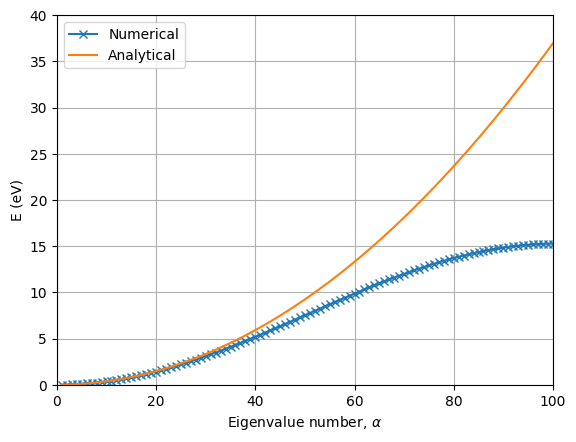
\includegraphics[scale=0.6]{discrete_PIB.png}
\end{figure}

\vspace{10pt}

The process of discretization did not yield an accurate analytical answer in this case since the setup itself is intrinsically continuous. However, for the problems we are interested in, this process yields fairly accurate solutions since the periodic nature of the lattice then facilitates its description as a discretized system. 

\subsection{Toy examples}

Consider a toy one-dimensional solid composed of $N$ atoms, separated by a distance $a$. Assuming one orbital per atom, the $N\times N$ Hamiltonian matrix can be written as follows:

\begin{equation}
H =
\begin{matrix}
     & \ket{1} & \ket{2} & \ldots & \ket{N-1} & \ket{N} \\
    \ket{1} & E_0 & E_{ss} & \ldots & 0 & E_{ss} \\
    \ket{2} & E_{ss} & E_0 & \ldots & 0 & 0 \\
    \vdots  &  &  &  &  &  \\
    \ket{N-1} & 0 & 0 & \ldots & E_0 & E_{ss} \\
    \ket{N} & E_{ss} & 0 & \ldots & E_{ss} & E_0 \\
\end{matrix}   
\end{equation}

The off-diagonal elements at the top-right and the bottom-left are to account for the fact that we are applying the \textit{periodic boundary condition}. The set of equations (all identical in form) that we obtain by applying $[H]\psi = E\psi$ can be written as ($n = 1, 2,\ldots N$)

\begin{equation*} \label{toy_prob}
    E\psi_{n} = E_0\psi_{n} + E_{ss}\psi_{n-1} + E_{ss}\psi_{n+1}
\end{equation*}

This set of equations can be solved analytically by the ansatz (via Bloch's Theorem):

\begin{equation} 
    \psi_{n} = \psi_0 e^{ikna} \quad \text{where} \quad ka = n2\pi/N
\end{equation}

Substituting the ansatz into \ref{toy_prob}, we obtain

\begin{equation}
    E = E_0 + 2E_{ss}cos(ka)
\end{equation}

\begin{figure}[!t]
\caption{\textit{Bandstructure for a one-dimensional solid with $E_0 = 0$ and $E_{ss} = -1$.}}\label{1d_chain}
\vspace{6pt}
\centering
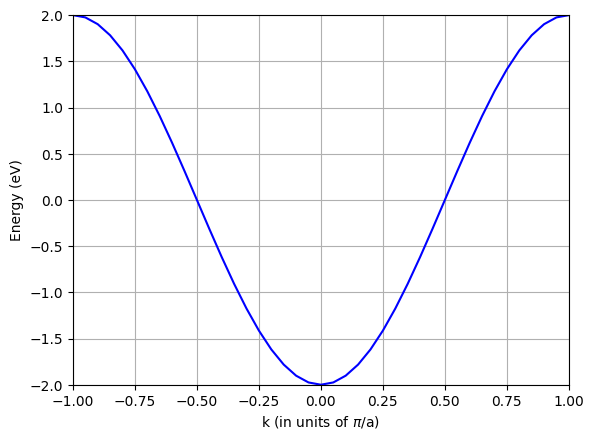
\includegraphics[scale=0.5]{1d_chain.png}
\end{figure}

It would seem logically inconsistent that while we started out with a $N \times N$ Hamiltonian and were expected to find $N$ discrete eigenvalues, we have instead found a continuous, periodic function apparently implying that we have infinitely many possible eigenvalues. Due to the discrete nature of the lattice, values of $ka$ that differ by $2\pi$ represent identical states, which can be verified by considering the ansatz ($k^{'} = k + 2\pi/a$):

\begin{equation}
\begin{aligned}
    \psi_{n}^{'} &= \psi_{0}e^{ik^{'}na} = \psi_{0}e^{ikna}e^{in2\pi} \\
    \psi_{n}^{'} &= \psi_{0}e^{ikna} = \psi_{n}
\end{aligned}
\end{equation}

Since only the values of $ka$ within a range of $2\pi$ yield independent solutions, in principle, we could take any range of size $2\pi$, and it would be physically acceptable. It is common to restrict $ka$ to the range $-\pi < ka < \pi$, otherwise known as the first Brillouin zone. Note that while we have now limited the possible eigenvalues within the first BZ, the continuous function seemingly implies that there are still infinitely many eigenvalues within the zone itself. This issue can be resolved by taking into consideration the periodic boundary condition applied to the Hamiltonian initially: $\psi_{0} = \psi_{N}$. This implies

\begin{equation}
\begin{aligned}
    \psi_{0} &= \psi_{N} = \psi_{0}e^{ikNa} \\
    ka &= \frac{2\pi}{N}\nu
\end{aligned}  
\end{equation}

where $\nu \in Z$. Thus, we end up with $N$ discrete energy eigenvalues, all bound within the first Brillouin zone, as intended initially. \par

Consider next a one-dimensional solid whose unit cell consists of two atoms as shown in Fig. \ref{peierls}.

\begin{figure}[!t]
\caption{\textit{A one-dimensional solid whose unit cell consists of two atoms.}}\label{peierls}
\centering
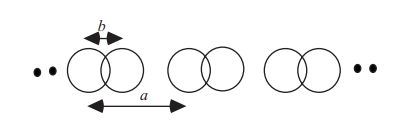
\includegraphics[scale=0.6]{peierls.png}
\end{figure}

Again, considering one orbital per atom, the matrix representation of the Hamiltonian is given by

\begin{equation}
H =
\begin{matrix}
     & \ket{1_A} & \ket{1_B} & \ket{2_A} & \ket{2_B} & \ket{3_A} & \ket{3_B} & \ldots\\
    \ket{1_A} & E_0 & E_{ss} & 0 & 0 & 0 & 0 & \ldots \\
    \ket{1_B} & E_{ss} & E_0 & E_{ss}^{'} & 0 & 0 & 0 & \ldots \\
    \ket{2_A} & 0 & E_{ss}^{'} & E_0 & E_{ss} & 0 & 0 & \ldots \\
    \ket{2_B} & 0 & 0 & E_{ss} & E_0 & E_{ss}^{'} & 0 & \ldots \\
    \ket{3_A} & 0 & 0 & 0 & E_{ss}^{'} & E_0 & E_{ss} & \ldots \\
    \ket{3_B} & 0 & 0 & 0 & 0 & E_{ss} & E_{0} & \ldots \\
\end{matrix}   
\end{equation}

Combine the elements of the matrix into ($2 \times 2$) blocks and rewrite it in the form

\begin{equation}
[H] =
\begin{matrix}
     & \ket{1} & \ket{2} & \ket{3} & \ldots \\
    \ket{1} & H_{11} & H_{12} & 0 & \ldots \\
    \ket{2} & H_{21} & H_{22} & H_{23} & \ldots \\
    \ket{3} & 0 & H_{32} & H_{33} & \ldots \\
\end{matrix}   
\end{equation}

where

\begin{equation*}
H_{nn} =
\begin{bmatrix}
    E_{0} & E_{ss} \\
    E_{ss} & E_{0} \\
\end{bmatrix}  \quad
H_{n,n+1} =
\begin{bmatrix}
    0 & 0 \\
    E_{ss}^{'} & 0 \\
\end{bmatrix}  \quad
H_{n,n-1} =
\begin{bmatrix}
    0 & E_{ss}^{'} \\
    0 & 0 \\
\end{bmatrix}  
\end{equation*}

The matrix equation ($[H]\psi = E\psi$) can be written in the form

\begin{equation}
    E\phi_n = H_{nn}\phi_n + H_{n,n-1}\phi_{n-1} + H_{n,n+1}\phi_{n+1}
\end{equation}

where $\{\phi_{n}\}$ represents a ($2 \times 1$) column vector (this is in accordance with the fact that we have two basis states). Yet again, the ansatz for solving this set of equations is given by

\begin{equation}
    \{\phi_n\} = \{\phi_0\}e^{ikna}
\end{equation}

Substituting the ansatz, we have

\begin{equation*}
    E\{\phi_0\} = H_{nn}\{\phi_0\} + H_{n,n-1}e^{-ika}\{\phi_0\} + H_{n,n+1}e^{ika}\{\phi_0\}
\end{equation*}

that is

\begin{equation*}
E\{\phi_0\} =
\begin{bmatrix}
    E_0 & E_{ss}+E_{ss}^{'}e^{-ika} \\
    E_{ss}+E_{ss}^{'}e^{ika} & E_0 \\
\end{bmatrix} \{\phi_0\}
\end{equation*}

The energy eigenvalues of the system are given by

\begin{equation}
    E = E_0 \pm \sqrt{E_{ss}^{2}+E_{ss}^{'2}+2E_{ss}E_{ss}^{'}cos(ka)}
\end{equation}

The $E(k)$ diagram for the solid is shown in Fig. \ref{ssh}. 

\begin{figure}[!t]
\caption{\textit{Bandstructure for the "dimerized" one-dimensional solid plotted using $E_{0} = 0, E_{ss} = 2, E_{ss}^{'} = 1$.}}\label{ssh}
\vspace{6pt}
\centering
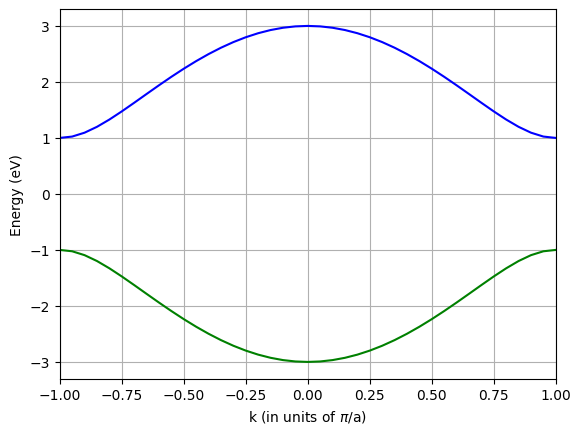
\includegraphics[scale=0.6]{ssh.png}
\end{figure}

It is energetically favourable for a uniform, one-dimensional chain of atoms, which we considered earlier to distort into the structure shown in Fig. \ref{peierls}-- a phenomenon referred to as \textit{Peierls' distortion}. 

\subsection{General result}

We shall now generalize this procedure for calculating the bandstructure of any periodic solid with an arbitrary number of basis functions per unit cell. Consider any particular unit cell $n$ connected to its neighboring unit cells $m$ by a Hamiltonian $[H_{nm}]$ of size $(b \times b)$, $b$ being the number of basis functions per unit cell. The overall matrix equation can be written as 

\begin{equation}
     E\{\phi_{n}\} = [H_{nm}]\{\phi_{m}\}
\end{equation} 

where $\{\phi_{m}\}$ is a ($b \times 1$) column vector denoting the wavefunction in unit cell $m$. The ansatz suggested for solving this is given by 

\begin{equation}
    \{\phi_{m}\} = \{\phi_{0}\}e^{i\vec{k}\cdot\vec{d_{m}}}
\end{equation}

Substituting the ansatz into the original matrix equation, we get

\begin{equation}
    E\{\phi_{0}\} = [h(\vec{k})]\{\phi_{0}\} \quad \text{with} \quad [h(\vec{k})] = \sum_{m}[H_{nm}]e^{i\vec{k}\cdot\vec{d_m}}
\end{equation}

The summation runs over all neighbouring unit cells (including itself) with which the unit cell $n$ has any overlap. In light of this, consider a 2-D lattice, which has been discretized into $M \times N$ points. Similar to the case of the 1-D chain, the first Brillouin zone is bound within $-\pi/a < k_x < +\pi/a$ and $-\pi/b < k_y < +\pi/b$.

\subsection{Graphene}

Graphene consists of a single layer of a hexagonal lattice of carbon atoms. The unit cell has to be chosen carefully in this case since adjacent carbon atoms aren't in an identical environment in the graphene lattice-- one of the atoms sees two neighbours to its right and one neighbour to the left, while the situation is vice-versa for the adjacent atom. But if we lump these two adjacent atoms into a unit cell as shown in Fig. \ref{graphene_lattice}, then the lattice of unit cells is periodic, and every site has an identical environment. 

\begin{figure}[!t]
\caption{\textit{Unit cell of two atoms in the graphene lattice.}}\label{graphene_lattice}
\vspace{4pt}
\centering
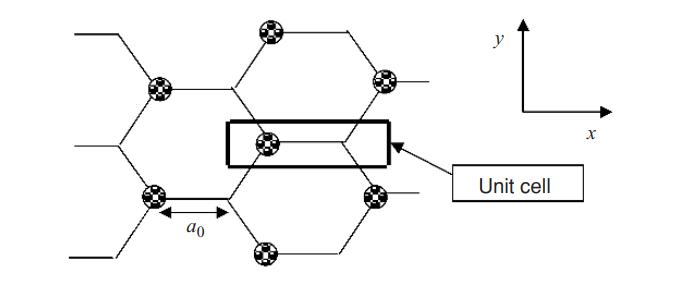
\includegraphics[scale=0.55]{graphene_lattice.png}
\end{figure}

It turns out that the 2$p_{z}$ orbital is sufficient to describe the bandstructure of graphene since the contribution of the 2$s$, 2$p_{x}$, and 2$p_{y}$ orbitals is insignificant in the vicinity of the Fermi energy. The resulting ($2 \times 2$) [$h(\vec{k})$] is given by 

\begin{align*}
    [h(\vec{k})] = 
    \begin{bmatrix}
        0 & -t \\
        -t & 0 
    \end{bmatrix} + 
    \begin{bmatrix}
        0 & -te^{i\vec{k}\cdot\vec{a_1}} \\ 
        0 & 0
    \end{bmatrix} + 
    \begin{bmatrix}
        0 & -te^{i\vec{k}\cdot\vec{a_2}} \\
        0 & 0
    \end{bmatrix} +  \\
    \begin{bmatrix}
        0 & 0 \\
        -te^{-i\vec{k}\cdot\vec{a_1}} & 0
    \end{bmatrix} + 
    \begin{bmatrix}
        0 & 0 \\
        -te^{-i\vec{k}\cdot\vec{a_2}} & 0 
    \end{bmatrix}  
\end{align*} 

where $\vec{a_1} = \hat{x}a+\hat{y}b, \quad \vec{a_2} = \hat{x}a-\hat{y}b$ with $a = 3a_{0}/2, \quad b = \sqrt{3}a_{0}/2 $. On simplifying the expression, 

\begin{equation}
[h(\vec{k})] =
    \begin{bmatrix}
        0 & h_{0} \\
        h_{0}^{*} & 0 
    \end{bmatrix}
\end{equation}

where $h_{0} = -t(1+2e^{ik_{x}a}cos(k_{y}b))$. The energy eigenvalues are given by 

\begin{equation}
    E = \pm |h_{0}| = \pm t\sqrt{1 + 4cos(k_{x}a)cos(k_{y}b) + 4cos^{2}(k_{y}b)}
\end{equation}

\begin{figure}[!htbp]
\caption{\textit{Bandstructure of graphene.}}\label{graphene_bands}
\vspace{2pt}
\centering
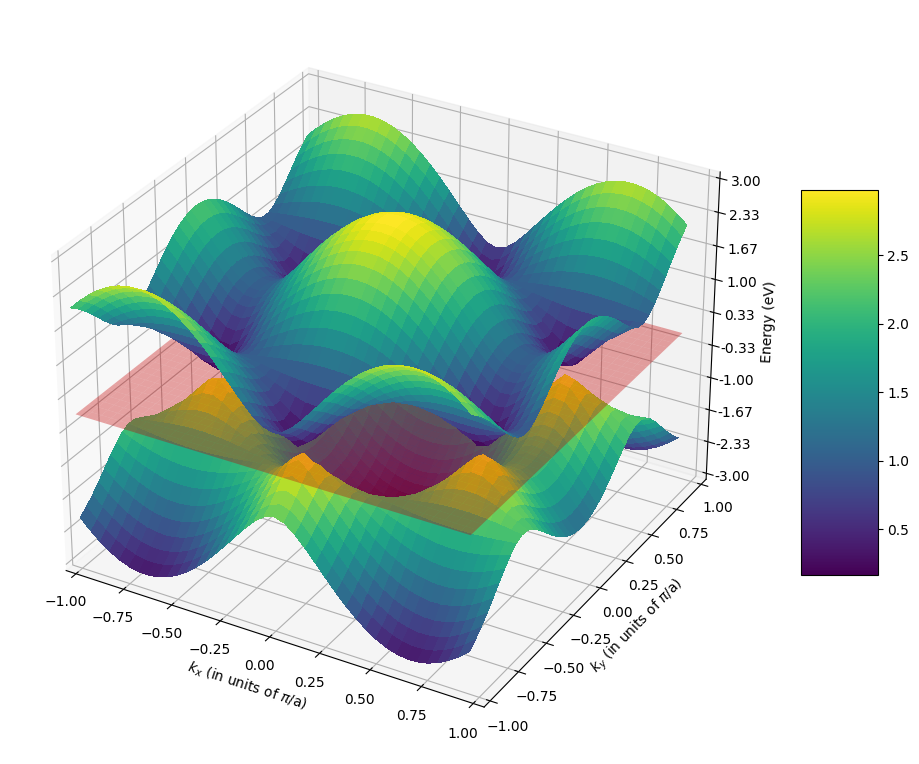
\includegraphics[scale=0.45]{graphene_bands.png}
\vspace{6pt}
\caption{\textit{Grayplots for the conduction band and valence band of graphene, respectively. Note the dark (or white) nodes which represent 'valleys' in the bandstructure.}}\label{graphene_grayplot}
\vspace{2pt}
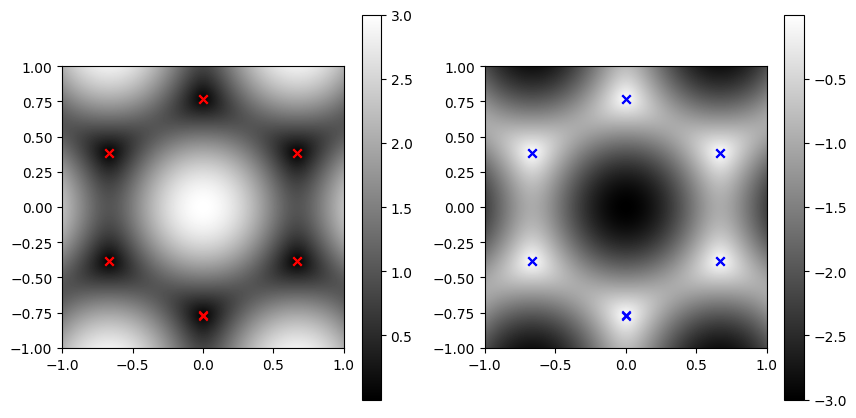
\includegraphics[scale=0.5]{graphene_grayplot.png}
\end{figure}

\newpage

\section{Epilogue}

While the current document encompasses a variety of topics, a significant volume of work remains to be done in Non-equilibrium Green functions (NEGF) formalism and the Bardeen-Cooper-Schreiffer (BCS) theory of superconductivity. I plan on adding content and simulations related to the same in the future, with my current target being running some fundamental NEGF simulations using the \textit{kwants} package while working on the theory of S-N, S-N-S, and N-S-N junctions alongside.  

\clearpage

\begin{thebibliography}{99} 
\bibitem{superconductivity} 
James Annett.
 \href{https://webuser.unicas.it/pagliarone/Super.pdf}{\textit{Superconductivity, Superfluids, and Condensates}}. 
Oxford University Press, 2004.

\bibitem{qt}
Supriyo Dutta.
 \href{https://www.cambridge.org/core/books/quantum-transport/E96BE74AACD59A03A7D6A7F7DACDFB71}{\textit{Quantum Transport - Atom to Transistor}}.
Cambridge University Press, 2005.

\bibitem{youtube_1}
Supriyo Dutta.
 \href{https://www.youtube.com/watch?v=eg4krA0xH6I}{\textit{Fundamentals of Nanoelectronics - Quantum Transport}}.
Youtube, 2015.

\bibitem{youtube_2}
Andrew Mitchell. 
 \href{https://www.youtube.com/playlist?list=PLotxEOxVaaoKRXdDN-7lI3Y88PaHqyOZL}{\textit{Quantum Condensed Matter Physics}}. 
Youtube, 2022.

\bibitem{youtube_3}
Nicola Spaldin. 
\href{https://www.youtube.com/playlist?list=PL8n8OkcK9SRZwL24mF7FeOa50Xd9YB-JO}{\textit{Schrödinger's Kittens Productions}}. Youtube, 2021.

\bibitem{ssh}
Navketan Batra and Goutam Sheet. 
 \href{https://link.springer.com/article/10.1007/s12045-020-0995-x}{\textit{Physics with Coffee and Doughnuts: Understanding the Physics Behind Topological Insulators Through Su-Schrieffer-Heeger Model}}.
Resonance, Indian Academy of Sciences, 2020.

\bibitem{bloch}
\href{https://bohr.physics.berkeley.edu/classes/221/s07/notes/blochban.pdf}{Lecture notes on Bloch's theorem}, 2005.

\bibitem{tight-binding}
\href{https://www.physics.rutgers.edu/~eandrei/chengdu/reading/tight-binding.pdf}{Lecture notes on tight binding models}, 2015.

\bibitem{second quantization}
Alexander Altland and Ben Simons.
\href{https://www.tcm.phy.cam.ac.uk/~bds10/tp3/secqu.pdf}{\textit{Quantum Condensed Matter Field Theory}}, 2023.
\end{thebibliography}

\end{document}